\section{Arc Length and Curvature} \label{S:9.8.Arc_Length_Curvature}

\vspace*{-14 pt}
\framebox{\hspace*{3 pt}
\parbox{6.25 in}{\begin{goals}
  \item How can a definite integral be used to measure the length of a
    curve in 2- or 3-space?
  \item Why is arc length useful as a parameter?
  \item What is the curvature of a curve?
\end{goals}} \hspace*{3 pt}}


\subsection*{Introduction}

Given a space curve, there are two natural
geometric questions one might ask: how long is the curve and how much
does it bend?  In this section, we answer both questions by
developing techniques for measuring the length of a space
curve as well as its curvature.

\begin{pa} \label{PA:9.8} In earlier investigations, we have used
  integration to calculate quantities such as area, volume, mass, and
  work.  We are now interested in determining the 
  length of a space curve.

  Consider the smooth curve in 3-space defined by the vector-valued
  function
    \[\vr(t) = \langle x(t), y(t), z(t) \rangle = \langle \cos(t), \sin(t), t \rangle\]
    for $t$ in the interval $[0,2\pi]$. Pictures of the graph of $\vr$ are shown in Figure \ref{F:9.8.Arc_length}.
  We will use the integration process to calculate the length of this curve. In this situation we partition the interval $[0,2\pi]$ into $n$ subintervals of equal length and let $0 = t_0 < t_1 < t_2 < \cdots < t_n = b$ be the endpoints of the subintervals. We then approximate the length of the curve on each subinterval with some related quantity that we can compute. In this case, we approximate the length of the curve on each subinterval with the length of the segment connecting the endpoints. Figure \ref{F:9.8.Arc_length} illustrates the process in three different instances using increasing values of $n$. 
\begin{figure}[ht]
\begin{center}
%\begin{minipage}{2.5in}
%\begin{center}
\resizebox{!}{1.5in}{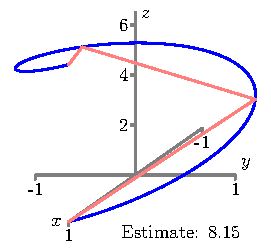
\includegraphics{figures/fig_9_8_length_animate_02.pdf}} \hspace{0.25in} \resizebox{!}{1.5in}{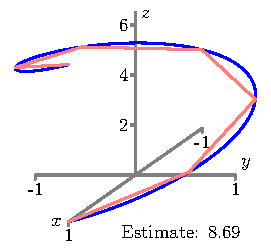
\includegraphics{figures/fig_9_8_length_animate_05.pdf}} \hspace{0.25in} \resizebox{!}{1.5in}{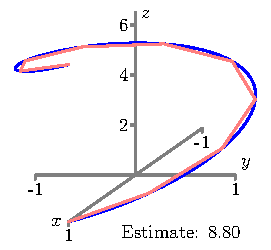
\includegraphics{figures/fig_9_8_length_animate_08.pdf}}
%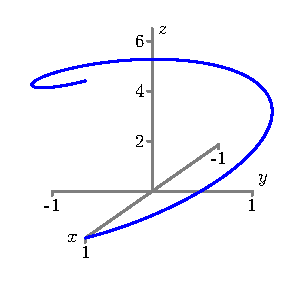
\includegraphics{figures/fig_9_8_length_1.eps}
%\end{center}
%\caption{The graph of $\vr$.}
%\label{F:9.8.Arc_length_3d}
%\end{minipage} \hspace{0.5in}
%\begin{minipage}{2.5in}
%\begin{center}
%\resizebox{!}{2.25in}{\animategraphics[controls,trim=0cm 0.0cm 0.25cm 1.5cm]{4}{9_8_AL3D_}{01}{20}}
%\animategraphics[controls]{2}{figures/fig_9_8_length_animate_}{00}{24}
\end{center}
\caption{Approximating the length of the curve with $n=3$, $n=6$, and $n=9$.}
\label{F:9.8.Arc_length}
%\label{F:9.8.Arc_length_3d_animation}
%\end{minipage}
%\end{center}
\end{figure}
%crop graphics in animate trim=<left> <bottom> <right> <top>, add, clip with \includegraphics
%Write the coordinates of the points on the curve determined by the endpoints of the interval $[x_{i-1},x_i]$.
    \ba
	\item Write a formula for the length of the line segment that connects the endpoints of the curve on the $i$th subinterval $[t_{i-1},t_i]$. (This length is our approximation of the length of the curve on this interval.) 
	
    \item Use your formula in part (a) to write a sum that adds all of the approximations to the lengths on each subinterval.

    \item What do we need to do with the sum in part (b) in order to obtain the exact value of the length of the graph of $\vr(t)$ on the interval $[0,2\pi]$?

    \ea


\end{pa} 


\begin{activitySolution}
   \ba
	\item The length of the line segment connecting the points $\vr(t_{i-1})$ and $\vr(t_i)$ is given by the distance formula
\[\sqrt{(x_i-x_{i-1})^2+(y_{i}-y_{i-1})^2 + (z_{i}-z_{i-1})^2}.\]

    \item We add the lengths given in part (b) to obtain the sum
\[\sum_{i=1}^n \sqrt{(x_i-x_{i-1})^2+(y_{i}-y_{i-1})^2 + (z_{i}-z_{i-1})^2}\]
that approximates the total length of the graph of $\vr(t)$ on the interval $[0,2 \pi]$.

    \item We must take the limit of the sum as $n$ goes to infinity.


    \ea
\end{activitySolution}


\afterpa 

\subsection*{Arc Length}

Consider a smooth curve in 3-space that is parametrically described by
the  vector-valued function $\vr$ defined by $\vr(t) = \langle x(t), y(t), z(t)
\rangle.$ 
Preview Activity
\ref{PA:9.8} shows that to approximate the
length of the curve defined by $\vr(t)$ as the values of $t$ run over
an interval $[a,b]$, we partition the interval $[a,b]$ into $n$
subintervals of equal length $\Delta t$, with $a = t_0 < t_1 < \cdots
< t_n = b$ as the endpoints of the subintervals. On each subinterval,
we approximate the length of the curve by the length of the line
segment connecting the endpoints. The points on the curve
corresponding to $t = t_{i-1}$ and $t = t_i$ are $(x(t_{i-1}),
y(t_{i-1}), z(t_{i-1}))$ and $(x(t_i), y(t_i), z(t_i))$, respectively,
so the length of the line segment connecting these points is
\[\sqrt{(x(t_i) - x(t_{i-1}))^2 + (y(t_i) - y(t_{i-1}))^2 + (z(t_i) -
  z(t_{i-1}))^2}.\]
Now we add all of these approximations together to obtain an
approximation to the length $L$ of the curve:
\[L \approx \sum_{i=1}^n \sqrt{(x(t_i) - x(t_{i-1}))^2 + (y(t_i) -
  y(t_{i-1}))^2 + (z(t_i) - z(t_{i-1}))^2}.\] 
We now want to take the limit of this sum as $n$ goes to infinity, but in its present form it
might be difficult to see how. We first introduce $\Delta t$ by multiplying by $\frac{\Delta t}{\Delta t}$, and see that 
\begin{align*}
L &\approx \sum_{i=1}^n \sqrt{(x(t_i) - x(t_{i-1}))^2 + (y(t_i) - y(t_{i-1}))^2 + (z(t_i) - z(t_{i-1}))^2} \\
    &= \sum_{i=1}^n \sqrt{(x(t_i) - x(t_{i-1}))^2 + (y(t_i) - y(t_{i-1}))^2 + (z(t_i) - z(t_{i-1}))^2} \frac{\Delta t}{\Delta t} \\
    &= \sum_{i=1}^n \sqrt{(x(t_i) - x(t_{i-1}))^2 + (y(t_i) - y(t_{i-1}))^2 + (z(t_i) - z(t_{i-1}))^2} \frac{\Delta t}{\sqrt{(\Delta t)^2}} 
\end{align*}
To get the difference quotients under the radical, we use properties of the square root function to see further that
\begin{align*}
L &\approx \sum_{i=1}^n \sqrt{\left[(x(t_i) - x(t_{i-1}))^2 + (y(t_i) - y(t_{i-1}))^2 + (z(t_i) - z(t_{i-1})^2\right] \frac{1}{(\Delta t)^2}} \Delta t \\
    &= \sum_{i=1}^n \sqrt{\left(\frac{x(t_i) - x(t_{i-1})}{\Delta t}\right)^2 + \left(\frac{y(t_i) - y(t_{i-1})}{\Delta t}\right)^2 + \left(\frac{z(t_i) - z(t_{i-1})}{\Delta t}\right)^2} \Delta t.
\end{align*}
Recall that as $n \to \infty$ we also have $\Delta t \to 0$. Since
\[\lim_{\Delta t \to 0} \frac{x(t_i) - x(t_{i-1})}{\Delta t} = x'(t), \ \lim_{\Delta t \to 0} \frac{y(t_i) - y(t_{i-1})}{\Delta t} = y'(t), \ \text{ and } \ \lim_{\Delta t \to 0} \frac{z(t_i) - z(t_{i-1})}{\Delta t} = z'(t)\]
we see that
\begin{align}
L &= \lim_{n \to \infty} \sum_{i=1}^n \sqrt{\left(\frac{x(t_i) - x(t_{i-1})}{\Delta t}\right)^2 + \left(\frac{y(t_i) - y(t_{i-1})}{\Delta t}\right)^2 + \left(\frac{z(t_i) - z(t_{i-1})}{\Delta t}\right)^2} \Delta t \notag \\
    &= \lim_{\Delta t \to 0} \sum_{i=1}^n \sqrt{\left(\frac{x(t_i) - x(t_{i-1})}{\Delta t}\right)^2 + \left(\frac{y(t_i) - y(t_{i-1})}{\Delta t}\right)^2 + \left(\frac{z(t_i) - z(t_{i-1})}{\Delta t}\right)^2} \Delta t \notag \\
    &= \int_a^b \sqrt{(x'(t))^2 + (y'(t))^2 + (z'(t))^2} \, dt. \label{eq:9.8.arclength_1}
\end{align}

Noting further that
\[|\vr'(t)| = \sqrt{(x'(t))^2 + (y'(t))^2 + (z'(t))^2},\]
we can rewrite (\ref{eq:9.8.arclength_1}) in a more succinct form as follows.

\vspace*{5pt}
\nin \framebox{\hspace*{3 pt}
\parbox{6.25 in}{If $\vr(t)$ defines a smooth curve $C$ on an interval $[a,b]$, then the \textbf{length}\index{arclength} $L$ of $C$ is given by
\begin{equation} \label{eq:9.8.arclength_2}
L = \int_a^b |\vr'(t)| \, dt.
\end{equation}
} \hspace*{3 pt}}
\vspace*{5pt}

Note that formula (\ref{eq:9.8.arclength_2}) applies to curves in any
dimensional space.  Moreover, this formula has a natural interpretation: if
$\vr(t)$ records the position of a moving object, then $\vr'(t)$ is
the object's velocity and $|\vr'(t)|$ its speed.  Formula
(\ref{eq:9.8.arclength_2}) says that we simply integrate the speed of
an object traveling over the curve to find the distance traveled by
the object, which is the same as the length of the curve,
just as in one-variable calculus.

\begin{activity} \label{A:9.8.1} Here we calculate the arc length of two familiar curves.
\ba
	\item Use Equation~(\ref{eq:9.8.arclength_2}) to calculate the circumference of a circle of radius $r$.
	\item Find the exact length of the spiral defined by $\vr(t) = \langle \cos(t), \sin(t), t \rangle$ on the interval $[0,2\pi]$. 
\ea	
\end{activity}
\begin{smallhint}

\end{smallhint}
\begin{bighint}

\end{bighint}
\begin{activitySolution}
\ba
	\item We can parameterize a circle of radius $r$ centered at the origin by $\vr(t) = \langle \cos(t), \sin(t) \rangle$ for $t$ in the interval $[0, 2\pi]$. The circumference of this circle is the length of curve defined by $r$, or
\[\int_0^{2\pi} \lvert \vr'(t) \rvert \, dt = \int_0^{2\pi} \sqrt{(-r\sin(t))^2 + (r\cos(t))^2} \, dt = \int_0^{2\pi} r \, dt = 2 \pi r\]
as expected.
	\item The length of curve defined by $r$ on the interval $[0,2 \pi]$ is 
\[\int_0^{2\pi} \lvert \vr'(t) \rvert \, dt = \int_0^{2\pi} \sqrt{(-\sin(t))^2 + (\cos(t))^2 + 1^2} \, dt = \int_0^{2\pi} \sqrt{2} \, dt = 2 \pi \sqrt{2}.\]
\ea
\end{activitySolution}

%%%%%%%%%%

\aftera



%\begin{activity} \label{A:9.8.2} Find the exact length of the spiral defined by $\vr(t) = \langle \cos(t), \sin(t), t \rangle$ on the interval $[0,2\pi]$. 


\end{activity}
\begin{smallhint}

\end{smallhint}
\begin{bighint}

\end{bighint}
\begin{activitySolution}
The length of curve defined by $r$ on the interval $[0,2 \pi]$ is 
\[\int_0^{2\pi} \lvert \vr'(t) \rvert \, dt = \int_0^{2\pi} \sqrt{(-\sin(t))^2 + (\cos(t))^2 + 1^2} \, dt = \int_0^{2\pi} \sqrt{2} \, dt = 2 \pi \sqrt{2}.\]
\end{activitySolution}
\aftera



We can adapt the arc length formula to curves in 2-space that define
$y$ as a function of $x$ as the following activity shows.

\begin{activity} \label{A:9.8.3} Let $y = f(x)$ define a smooth curve in 2-space. Parameterize this curve and use Equation~(\ref{eq:9.8.arclength_2}) to show that the length of the curve defined by $f$ on an interval $[a,b]$ is
\[\int_a^b \sqrt{1+[f'(t)]^2} \, dt.\]


\end{activity}
\begin{smallhint}

\end{smallhint}
\begin{bighint}

\end{bighint}
\begin{activitySolution}
We can parameterize $y=f(x)$ on $[a,b]$ by $\vr(t) = \langle t, f(t) \rangle$ for $t$ in $[a,b]$. Then the length of the curve defined by $y=f(x)$ on $[a,b]$ is
\[\int_a^b \lvert \vr'(t) \rvert \, dt =  \int_a^b \lvert \langle 1, f'(t) \rvert \, dt = \int_a^b \sqrt{1+[f'(t)]^2} \, dt.\]
\end{activitySolution}
\aftera


\subsection*{Parameterizing With Respect To Arc Length}

In addition to helping us to find the length of space curves, the
expression for the length of a curve enables us to find a natural
parametrization of space curves in terms of arc length, as we now
explain. 

Shown below in Figure \ref{F.9.8.parametrization} is a portion of the
parabola $y = x^2/2$.  Of course, this space curve may be parametrized by 
the vector-valued function $\vr$ defined by $\vr(t) = \langle t, t^2/2\rangle$ as shown
on the left, where we see the location at a few different times $t$.
Notice that the points are not equally spaced on the curve.

A more natural parameter describing the points along the space curve
is the distance traveled $s$ as we move along the parabola starting at
the origin.  For instance, the right side of Figure
\ref{F.9.8.parametrization} shows the points corresponding to various
values of $s$.  We call this an {\em arc length parametrization}.

\begin{figure}[ht]
  \begin{center}
    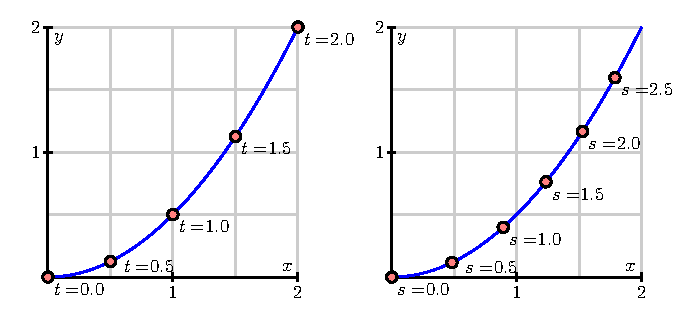
\includegraphics{figures/fig_9_8_param.eps}
    \caption{The parametrization $\vr(t)$ (left) and a
      reparametrization by arc length.}
    \label{F.9.8.parametrization}
  \end{center}
\end{figure}

To see that this is a more natural parametrization, consider an
interstate highway cutting across a state.  One way
to parametrize the curve defined by the highway is to drive along the
highway and record our position at every time, thus creating a
function $\vr$.  If we encounter an accident or road construction,
however,
this parametrization might not be at all relevant to another person
driving the same highway.  An arc length parametrization, however, is
like using the mile markers on the side of road to specify our
position on the highway.  If we know how far we've traveled along the
highway, we know exactly where we are.

If we begin with a parametrization of a space curve, we can
modify it to find an arc length parametrization, as we now describe.
Suppose that the curve is parametrized by the vector-valued function
$\vr = \vr(t)$ where $t$ is in the interval $[a,b]$.  We define the
parameter $s$ through the function
\[s=L(t) = \int_a^t \sqrt{(x'(w))^2 + (y'(w))^2 + (z'(w))^2} \,dw,\] 
which measures the length along the curve from $\vr(a)$ to
$\vr(t)$.  

The Fundamental Theorem of Calculus shows us that
\begin{equation} \label{eq:9.8.arc_length_prime} \frac{ds}{dt} =
  L'(t)=
  \sqrt{(x'(t))^2 + (y'(t))^2 + (z'(t))^2} = \lvert \vr'(t) \rvert
\end{equation}
and so
\[L(t) = \int_a^t \left| \frac{d}{dt}\vr(w)\right| \,dw.\] 
If we assume that $\vr'(t)$ is never 0, then $L'(t) > 0$ for all $t$
and $s=L(t)$ is always increasing. This should seem reasonable: unless we
stop, the distance traveled along the curve increases as we move along
the curve.

Since $s=L(t)$ is an increasing function, it is invertible, which means
we may view the time $t$ as a function of the distance traveled;  that
is, we have the relationship $t=L^{-1}(s)$.  We then obtain the arc length
parametrization by composing $\vr(t)$ with $t=L^{-1}(s)$ to obtain
$\vr(s)$.  Let's illustrate this with an example.

\begin{example} \label{ex:9.8.circle_arc_length} Consider a circle of
  radius $5$ in 2-space centered at the origin. We know that we can
  parameterize this circle as
  \[\vr(t) = \langle 5\cos t, 5\sin t \rangle, \]
  where $t$ runs from 0 to $2\pi$.  
  We see that $\vr'(t) = \langle -5\sin t, 5\cos t\rangle$, and hence
  $|\vr'(t)| = 5$.  It then follows that
  $$
  s=L(t) = \int_0^t |\vr'(w)|~dw = \int_0^t 5~dw = 5t.
  $$
  Since $s=L(t) = 5t$, we may solve for $t$ in terms of $s$ to obtain
  $t=L^{-1}(s) 
  = s/5$.  We then find the arc length parametrization by composing
  \[\vr(s)=\vr(L^{-1}(s)) = \left\langle 5\cos\left(\frac s5\right),
  5\sin\left(\frac s5\right)\right\rangle.\]


More generally, for a circle of radius $a$ centered at the origin, a
similar computation shows that
\begin{equation}
\vr(s) = \left\langle a\cos\left(\frac sa\right), a\sin\left(\frac sa\right)\right\rangle
\label{eq:9.8.circle_arc_length_parameterization}
\end{equation}
is an arc length parametrization.

\end{example}

Notice that equation (\ref{eq:9.8.arc_length_prime}) shows that 
\[\frac{d\vr}{dt} = \frac{d\vr}{ds}\frac{ds}{dt} = \frac{d\vr}{ds}\lvert \vr'(t) \rvert,\]
so
\[\left| \frac{d\vr}{ds} \right| = \left|\frac{1}{\lvert \vr'(t) \rvert}\frac{d\vr}{dt} \right| = 1,\]
which means that we move along the curve with unit speed when we parameterize by arc length. This is clearly seen in Example \ref{ex:9.8.circle_arc_length} where $|\vr'(s)| = 1$. It follows that the parameter $s$ 
is the distance traveled along the curve, as shown by:
$$
L(s) = \int_0^s\left|\frac{d}{ds}\vr(w)\right|~dw = \int_0^s1~dw = s.
$$

\begin{activity} \label{A:9.8.4} In this activity we parameterize a
  line in 2-space in terms of arc length. Consider the line with
  parametric equations
\[x(t) = x_0+at \ \ \ \ \text{ and } \ \ \ \ y(t) = y_0+bt.\]
    \ba
    \item To write $t$ in terms of $s$, evaluate the integral
    \[s=L(t) = \int_{0}^t \sqrt{(x'(w))^2 + (y'(w))^2} \, dw\]
    to determine the length of the line from time 0 to time $t$.

  \item Use the formula from (a) for $s$ in terms of $t$ to write $t$
    in terms of $s$. Then explain why a parameterization of the line
    in terms of arc length is
 \begin{equation} \label{eq:9.8.line_arc_length_parameterization}
x(s) = x_0+\frac{a}{\sqrt{a^2+b^2}}s \ \ \ \ \text{ and } \ \ \ \ y(s) = y_0+\frac{b}{\sqrt{a^2+b^2}}s.
\end{equation}

    \ea

\end{activity}
\begin{smallhint}

\end{smallhint}
\begin{bighint}

\end{bighint}
\begin{activitySolution}
\ba
\item The length of the line from time 0 to time $t$ is 
\begin{align*}
s(t) &= \int_{0}^t \sqrt{(x'(w))^2 + (y'(w))^2} \, dw \\
    &= \int_0^t \sqrt{a^2+b^2} \, dw \\
    &= \sqrt{a^2+b^2}t.
\end{align*}
\item We have $t = \frac{s}{\sqrt{a^2+b^2}}$, and so a parameterization for the line in terms of arc length is
\[x(s) = x_0+\frac{a}{\sqrt{a^2+b^2}}s \ \ \ \ \text{ and } \ \ \ \ y(s) = y_0+\frac{b}{\sqrt{a^2+b^2}}s.\]
\ea
\end{activitySolution}
\aftera


A little more complicated example is the following.

\begin{example} \label{ex:9.8.AL_curvature_ex_2}  Let us parameterize the curve defined by
\[\vr(t) = \left\langle t^2, \frac{8}{3}t^{3/2}, 4t \right\rangle\]
for $t \geq 0$ in terms of arc length. To write $t$ in terms of $s$ we find $s$ in terms of $t$:
\begin{align*}
s(t) &= \int_{0}^t \sqrt{(x'(w))^2 + (y'(w))^2 +(z'(w))^2} \, dw \\
    &= \int_0^t \sqrt{(2w)^2 + (4w^{1/2})^2 + (4)^2} \, dw \\
    &= \int_0^t \sqrt{4w^2 + 16w + 16} \, dw \\
    &= 2\int_0^t \sqrt{(w+2)^2} \, dw \\
    &= 2\int_0^t w+2 \, dw \\
    &= \left(w^2+4w\right)\biggm|_{0}^{t} \\
    &= t^2+4t.
\end{align*}
Since $t \geq 0$, we can solve the equation $s = t^2+4t$ (or $t^2+4t-s=0$) for $t$ to obtain $t = \frac{-4 +\sqrt{16+4s}}{2} = -2 + \sqrt{4+s}$. So we can parameterize our curve in terms of arc length by
\[\vr(s) = \left\langle \left(-2 + \sqrt{4+s}\right)^2, \frac{8}{3}\left(-2 + \sqrt{4+s}\right)^{3/2}, 4\left(-2 + \sqrt{4+s}\right) \right\rangle.\]

\end{example}

These examples illustrate a general method.  Of course, evaluating an
arc length integral and finding a formula for the
inverse of a function can be difficult, so while this process is
theoretically possible, it is not always practical to parameterize a
curve in terms of arc length. However, we can guarantee that such a
parameterization exists, and this observation plays an important role
in the next section. 

\subsection*{Curvature}

For a smooth space curve, the \emph{curvature} measures how fast the
curve is bending or changing direction at a given point. For example,
we expect that a line should have zero curvature everywhere, while a
circle (which is bending the same at every point) should have constant
curvature.  Circles with larger radii should have smaller curvatures.

To measure the curvature, we first need to describe the direction of
the curve at a point.  We may do this using a continuously varying
tangent vector to the curve, as shown in \ref{F:9.8.Curvature_1}.  
The direction of the curve is then determined by the angle $\phi$ this
tangent vector makes with a horizontal vector, as shown in
\ref{F:9.8.Curvature_angles}.  

\begin{figure}[ht]
\begin{center}
\begin{minipage}{3in}
\begin{center}
%\resizebox{!}{1.5in}{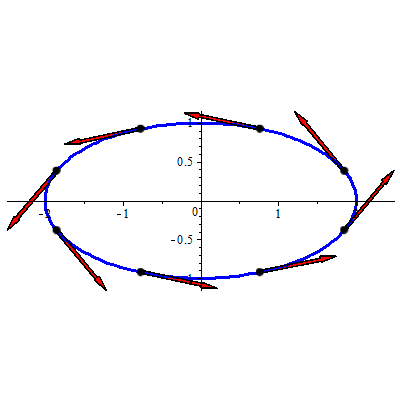
\includegraphics[trim=0cm 3.25cm 0cm 3.25cm,
%clip]{9_8_Curvature_1}}
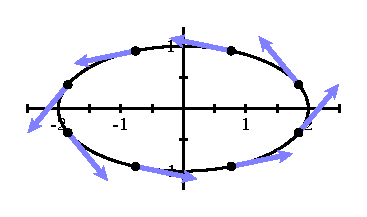
\includegraphics{figures/fig_9_8_tangents.eps}
\end{center}
\caption{Tangent vectors to an ellipse.}
\label{F:9.8.Curvature_1}
\end{minipage} %\hspace{0.5in}
\begin{minipage}{3in}
\begin{center}
%\resizebox{!}{1.5in}{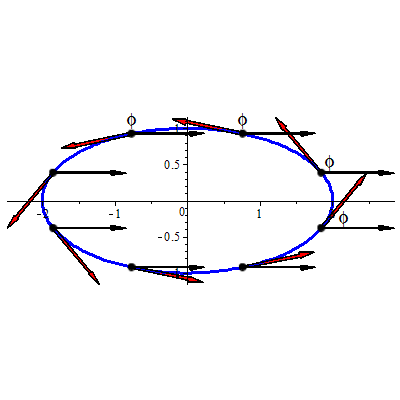
\includegraphics[trim=0cm 3.25cm 0cm 3.25cm, clip]{9_8_Curvature_angles}}
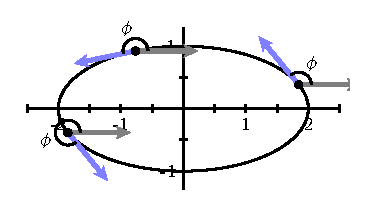
\includegraphics{figures/fig_9_8_tangents_angles.eps}
\end{center}
\caption{Angles of tangent vectors.}
\label{F:9.8.Curvature_angles}
\end{minipage}
\end{center}
\end{figure}

Informally speaking, the curvature will be
the rate at which the angle $\phi$ is changing as we move along the
curve.  Of course, this rate of change will depend on how we move
along the curve;  if we move with a greater speed along the curve,
then $\phi$ will change more rapidly.  This is why the speed limit is
sometimes lowered when we enter a curve on a highway.  In other words,
the rate of change of $\phi$ will depend on the parametrization we use
to describe the space curve.  To eliminate this dependence on the
parametrization, we choose to work with an arc
length parametrization $\vr(s)$, which means we move along the curve
with unit speed. 

Using an arc length parametrization $\vr(s)$, we define the tangent vector
$\vT(s) = \vr'(s)$, and note that $|\vT(s)| = 1$;  that is, $\vT(s)$ is
a unit tangent vector.  We then have $\vT(s) = \langle \cos (\phi(s)),
\sin(\phi(s)) \rangle$, 
which means that
$$\frac{d\vT}{ds} = \left\langle -\sin(\phi(s)) \frac{d\phi}{ds}, ~
\cos(\phi(s)) \frac{d\phi}{ds} \right\rangle = 
\langle -\sin(\phi(s)),~
\cos(\phi(s)) \rangle \frac{d\phi}{ds}.
$$
Therefore
$$\left|\frac{d\vT}{ds}\right| =  \left|\langle -\sin(\phi(s)),~
\cos(\phi(s)) \rangle\right| ~\left|\frac{d\phi}{ds}\right| = 
\left|\frac{d\phi}{ds}\right|$$.

This observation leads us to adopt 

\vspace*{5pt}
\nin \framebox{\hspace*{3 pt}
\parbox{6.25 in}{\begin{definition} If $C$ is a smooth space curve and
    $s$ is an arc length parameter for $C$, then the \textbf{curvature}\index{curvature}, $\kappa$,\footnote{$\kappa$ is the Greek lowercase letter ``kappa".} of $C$ is
\[\kappa = \kappa(s) = \left\lvert \frac{d \vT}{ds} \right\rvert.\] \end{definition}
} \hspace*{3 pt}}
\vspace*{5pt}

% We may describe the direction of the curve at a point using a unit
% tangent vector.  That is, at a point on the curve, $\vT$ will be a
% vector tangent to the curve having unit length, as shown in Figure
% \ref{F:9.8.Curvature_1}.  Of course, there are two choices of the unit
% tangent vector at every point;  we simple choose the 

% A natural place to start to think about measuring curvature is to
% determine how fast the tangent vector is changing, or $|\vv'(t)|$, as
% illustrated in Figure \ref{F:9.8.Curvature_1}. However, $\vv'(t)$ is a
% function of time, and curvature should not depend on how fast we are
% traveling along the curve. How the curve is bending should be
% independent of how fast we travel along the curve. Think about driving
% a car around a curve -- the curve is the same regardless of how fast
% we drive, but you can feel the effect of the curve more if you drive
% through it faster. We need a way to measure curvature that does not
% depend on speed or parameterization. A next logical step is to try to
% remove the dependence on speed by making the speed constant, that is
% normalizing the velocity vector and consider using the \emph{unit
%   tangent vector}
% \[\vT(t) = \frac{\vv(t)}{\lvert \vv(t) \rvert}.\]
% We might then try to use $\lvert \vT'(t) \rvert$ as a measure of
% curvature. But this, too, has its problems. To see why, note that
% $\vr_1(t) = \langle t, t^2 \rangle$ and $\vr_2(t) = \langle 2t, 4t^2
% \rangle$ are two parameterizations of the parabola $y=x^2$. Their
% respective velocity vectors are $\vv_1(t) = \langle 1,2t\rangle$ and
% $\vv_2(t) = \langle 2, 8t \rangle$ and the respective unit tangent
% vectors are $\vT_1(t) = \frac{1}{\sqrt{1+4t^2}} \langle 1,2t\rangle$
% and $\vT_2(t) = \frac{1}{\sqrt{1+16t^2}} \langle 1,4t\rangle$. It
% follows that
% \[\left\lvert \vT'_1(t) \right\rvert = \frac{2}{1+4t^2} \ \ \ \text{ and } \ \ \ \left\lvert \vT'_2(t) \right\rvert = \frac{4}{1+16t^2}.\]
% Now the point $(1,1)$ is the terminal point of $\vr_1(1)$ and $\vr_2\left(\frac{1}{2}\right)$, so we should expect the curvature of this curve to be the same whether we use the parameterization $\vr_1$ or $\vr_2$. But
% \[\frac{2}{1+4(1)^2} = \frac{2}{5} \ \ \ \text{ and } \ \ \ \frac{4}{1+16\left(\frac{1}{2}\right)^2} = \frac{4}{5}.\]
% So the value of  $\lvert \vT'(t) \rvert$ at a point depends on the parameterization we use. In other words, we still haven't removed the dependence on  how fast we travel along a curve. That is, $\lvert \vT'(t) \rvert$ still depends on the parameterization we choose.

% To remove the dependence of our computations on the parameterization, we need to take a different approach -- one that relies only on the geometric properties of the curve. A perfect method for this it to use the arc length parameterization discussed in the previous section. Even if we have different parameterizations of a curve, we travel the same distance when we move along the curve from point $P$ to point $Q$ regardless of how fast we go. In other words, arc length is independent of the parameterization, so arc length is the kind of parameter we want.

% %crop graphics in animate trim=<left> <bottom> <right> <top>, add, clip with \includegraphics

% We still want to measure the change in the unit tangent vectors, but the key is to parameterize the tangent vectors in terms of arc length. The magnitude of the change in the unit tangent vector with respect to arc length will tell us how fast the unit tangent vector is changing as the arc length changes, giving us a measure of the bend in the curve that does not depend on the parameterization. This is how we define curvature.

\begin{example} We should expect that the curvature of a line is 0
  everywhere. To show that our definition of curvature measures this
  correctly in 2-space, recall that
  (\ref{eq:9.8.line_arc_length_parameterization}) gives us the arc
  length parameterization
  \[x(s) = x_0+\frac{a}{\sqrt{a^2+b^2}}s \ \ \ \ \text{ and } \ \ \ \
  y(s) = y_0+\frac{b}{\sqrt{a^2+b^2}}s\] of a line. So the unit tangent vector is 
\[\vT(s) = \left\langle \frac{a}{\sqrt{a^2+b^2}},
  \frac{b}{\sqrt{a^2+b^2}} \right\rangle\] 
and, since $\vT(s)$ is constant, we have
\[\kappa = \left\lvert \frac{d \vT}{ds} \right\rvert = 0\]
as expected.
\end{example}

\begin{activity} \label{A:9.8.5} Recall that an arc length
  parameterization of a circle in 2-space of radius $a$ centered at
  the origin is, from
  (\ref{eq:9.8.circle_arc_length_parameterization}),
  \[\vr(s) = \left\langle a \cos\left(\frac{s}{a}\right),~
    a \sin\left(\frac{s}{a}\right)\right\rangle.\] 
    Show that the curvature
    of this circle is the constant $\frac{1}{a}$. What can you say about the relationship between the size of the radius of a circle and the value of its curvature?  Why does this make sense?

\end{activity}
\begin{smallhint}

\end{smallhint}
\begin{bighint}

\end{bighint}
\begin{activitySolution}
We have
\[\vT(s) = \left\langle -\sin\left(\frac{s}{a}\right), \cos\left(\frac{s}{a}\right) \right\rangle.\]
So the curvature of a circle of radius $a$ is
\begin{align*}
\kappa &= \left\lvert \frac{d \vT}{ds} \right\rvert \\
    &= \left\lvert \left\langle -\frac{1}{a}\cos\left(\frac{s}{a}\right), -\frac{1}{a}\sin\left(\frac{s}{a}\right) \right\rangle \right\rvert \\
    &= \frac{1}{a}.
\end{align*}
So, as expected, larger circles have smaller curvature.
\end{activitySolution}
\aftera


The definition of curvature relies on our
ability to parameterize curves in terms of arc length. Since we have
seen that finding an arc length parametrization can be difficult, we
would like to be able to express the curvature in terms of a more
general parametrization $\vr(t)$.

To begin, we need to describe the vector $\vT$, which is
a vector tangent to the curve having unit length.  Of course, the
velocity vector $\vr'(t)$ is tangent to the curve;  we simply need to
normalize its length to be one.  This means that we may take
$$
\vT(t) = \frac{\vr'(t)}{|\vr'(t)|}.
$$

Then the curvature of the curve defined by $\vr$ is
\begin{align*}
\kappa &= \left\lvert \frac{d \vT}{ds} \right\rvert \\
    &= \left\lvert \frac{d \vT}{dt} \frac{dt}{ds} \right\rvert \\
    &= \frac{\left\lvert \frac{d \vT}{dt} \right\rvert}{ \left\lvert \frac{ds}{dt} \right\rvert } \\
    &= \frac{\left\lvert \vT'(t) \right\rvert}{ \left\lvert \vr'(t) \right\rvert}.
\end{align*}

This last formula allows us to use any parameterization of a curve to
calculate its curvature. There is another useful formula, given
below, whose derivation is left for the exercises.

\vspace*{5pt}
\nin \framebox{\hspace*{3 pt}
  \parbox{6.25 in}{If $\vr(t)$ is a vector-valued function defining a
    smooth space curve $C$, and if $\vr'(t)$ is not
    zero and if $\vr''(t)$ exists, then the curvature $\kappa$ of $C$
    satisfies
\begin{itemize}
\item $\kappa = \kappa(t) = \frac{\left\lvert \vT'(t) \right\rvert}{ \left\lvert \vr'(t) \right\rvert}$
\item $\kappa = \frac{\lvert \vr'(t) \times \vr''(t) \rvert}{\lvert \vr'(t) \rvert^3}$.
\end{itemize}
} \hspace*{3 pt}}
\vspace*{5pt}

\begin{activity} \label{A:9.8.6} Use one of the two formulas for $\kappa$ in terms of $t$ to help you answer the following questions.
\ba
	\item The ellipse $\frac{x^2}{a^2} + \frac{y^2}{b^2} = 1$ has parameterization
\[\vr(t) = \langle a\cos(t), b\sin(t) \rangle.\]
Find the curvature of the ellipse. Assuming $0 < b < a$, at what points is the curvature the greatest and at what points is the curvature the smallest? Does this agree with your intuition?
	\item The standard helix has parameterization $\vr(t) = \cos(t) \vi + \sin(t) \vj + t \vk$.  Find the curvature of the helix.  Does the result agree with your intuition?
\ea
\end{activity}
\begin{smallhint}

\end{smallhint}
\begin{bighint}

\end{bighint}
\begin{activitySolution}
\ba
	\item We have
\[\vT(t) = \left\langle -\frac{a\sin(t)}{\sqrt{a^2\sin^2(t) + b^2\cos^2(t)}}, \frac{b\cos(t)}{\sqrt{a^2\sin^2(t) + b^2\cos^2(t)}} \right\rangle\]
and
\[\vT'(t) = \left\langle -\frac{ab^2\cos(t)}{\left(a^2\sin^2(t) + b^2\cos^2(t)\right)^{3/2}}, -\frac{a^2b\sin(t)}{\left(a^2\sin^2(t) + b^2\cos^2(t)\right)^{3/2}} \right\rangle.\]
So the curvature of the ellipse is given by
\begin{align*}
\kappa(t) &= \frac{1}{\left(a^2\sin^2(t) + b^2\cos^2(t)\right)^2} \sqrt{(ab^2\cos(t))^2 +(a^2b\sin(t))^2} \\
    &= \frac{ab}{\left(a^2\sin^2(t) + b^2\cos^2(t)\right)^2} \sqrt{b^2\cos^(t) + a^2\sin^2(t)} \\
    &= \frac{ab}{\left(a^2\sin^2(t) + b^2\cos^2(t)\right)^{3/2}}.
\end{align*}
If we assume that $0 < b < a$, then we should expect that ellipse to have the largest curvature at the points $(\pm a, 0)$ and the smallest at the points $(0, \pm b)$ (when $t = \frac{\pi}{2} + \pi k$ for some integer $k$). The denominator of our curvature function can be written as
\[a^2(1-\cos^2(t)) + b^2 \cos^2(t) = a^2 - (a^2-b^2)\cos^2(t).\]
The curvature of the ellipse is largest when this denominator is smallest, or when $t = 0$ or $t=\pi$. These $t$ values correspond to the points $(\pm a, 0)$. Similarly, the curvature of the ellipse is smallest when the denominator is largest, or when $t = \frac{\pi}{2}$ and $t = \frac{3\pi}{2}$. These $t$ values correspond to the points $(0, \pm b)$ as expected.
	\item Here we have
\[\vr'(t) = (-\sin(t)) \vi + \cos(t) \vj + \vk\]
and
\[\vT(t) = \frac{1}{\sqrt{2}}\left( (-\sin(t)) \vi + \cos(t) \vj + \vk \right).\]
Then
\[\vT'(t) = \frac{1}{\sqrt{2}}\left( (-\cos(t)) \vi - \sin(t) \vj \right)\]
and so
\[\kappa(t) = \frac{1}{2}.\]
\ea
\end{activitySolution}
\aftera


%%%%%%%%%%%%%%%%%%%%%






%Of course, we can calculate curvature in 3-space.

%\begin{activity} \label{A:9.8.7} Find the curvature of the helix with parameterization $\vr(t) = \cos(t) \vi + \sin(t) \vj + t \vk$.

\end{activity}
\begin{smallhint}

\end{smallhint}
\begin{bighint}

\end{bighint}
\begin{activitySolution}
Here we have
\[\vr'(t) = (-\sin(t)) \vi + \cos(t) \vj + \vk\]
and
\[\vT(t) = \frac{1}{\sqrt{2}}\left( (-\sin(t)) \vi + \cos(t) \vj + \vk \right).\]
Then
\[\vT'(t) = \frac{1}{\sqrt{2}}\left( (-\cos(t)) \vi - \sin(t) \vj \right)\]
and so
\[\kappa(t) = \frac{1}{2}.\]
\end{activitySolution}
\aftera


The curvature has another interpretation.  Recall that the tangent
line to a curve at a point is the line that best approximates the
curve at that point.  The curvature at a point on a curve describes
the {\em circle} that best approximates the curve at that point.
Remembering that a circle of radius $a$ has curvature $1/a$, then the
circle that best approximates the curve near a point on a curve whose
curvature is $\kappa$ has radius $1/\kappa$ and will be tangent to the
tangent line at that point.  This circle, called the {\em osculating
  circle} of the curve at the point, is shown in Figure
\ref{F:9.8.osculating} for a portion of a
parabola.

\begin{figure}[ht]
  \begin{center}
    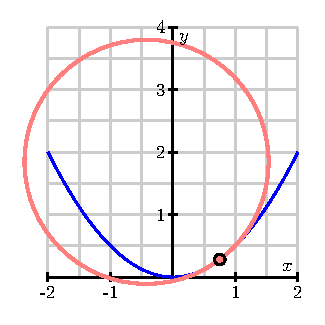
\includegraphics{figures/fig_9_8_curvature.eps}
    \caption{The osculating circle}
    \label{F:9.8.osculating}
  \end{center}
\end{figure}

% We can interpret curvature in 2-space in an interesting way. Let $\vr(t)$ define a smooth curve in $\R^2$ and let $\phi$ be the angle that the tangent vector $\vr'(t)$ makes with the vector $\vi$, as shown in Figure \ref{F:9.8.Curvature_angles}. If $\vT$ is a unit tangent vector to the curve where $\phi$ is the angle between $\vT$ and $\vi$, then we can write $\vT$ as
% \[\vT = \langle \cos(\phi), \sin(\phi) \rangle.\]
% As a result, we have
% \[\frac{d \vT}{ds} = \frac{d \vT}{d \phi} \frac{d \phi}{ds},\]
% so
% \begin{align*}
% \kappa &= \left\lvert \frac{d \vT}{ds} \right\rvert \\
%     &= \left\lvert \frac{d \vT}{d \phi} \right\rvert \ \left\lvert \frac{d \phi}{ds} \right\rvert \\
%     &= \left\lvert \langle -\sin(\phi), \cos(\phi) \right\rvert \ \left\lvert \frac{d \phi}{ds} \right\rvert \\
%     &= \sqrt{\sin^2(\phi) + \cos^2(\phi)} \left\lvert \frac{d \phi}{ds} \right\rvert \\
%     &= \left\lvert \frac{d \phi}{ds} \right\rvert.
% \end{align*}

% So the curvature of a curve in 2-space is also a measure of how the angle between the tangent vectors and the positive $x$-axis is changing as we move along the curve.


\begin{summary}
\item The integration process shows that the length $L$ of a smooth curve defined by $\vr(t)$ on an interval $[a,b]$ is
\[L = \int_a^b |\vr'(t)| \, dt.\]
\item Arc length is useful as a parameter because when we parameterize with respect to arc length, we eliminate the role of speed in our calculation of curvature and the result is a measure that depends only on the geometry of the curve and not on the parameterization of the curve.
\item We define the curvature $\kappa$ of a curve in 2- or 3-space to be the rate of change of the unit tangent vector with respect to arc length, or
    \[\kappa = \left\lvert \frac{d\vT}{ds} \right\rvert.\]
\end{summary}


%Potential Exercises

%Show that the curvature of a curve with parameterization $\vr(t)$ in $R^3$ can be found by
%\[\kappa = \frac{\lvert \vr'(t) \times \vr''(t) \rvert}{\lvert \vr'(t) \rvert^3}.\]


%Note that if $\vr(s)$ defines a curve as a function of arc length $s$, then equation (\ref{eq:arc_length_prime}) shows that
%\[\frac{d\vr}{ds} = \frac{d \vr}{dt} \frac{dt}{ds} = \frac{d \vr/dt}{ds/dt} = \frac{\vr'(t)}{|\vr'(t)|} = \vT(t),\]
%so $\frac{d\vr}{ds}$ is the unit tangent vector.


\nin \hrulefill

\begin{exercises} 

\item \label{Ez:9.8.1}    Consider the moving particle whose position at time $t$ in seconds is given by the vector-valued function $\vr$ defined by $\vr(t) = 5t \vi + 4\sin(3t) \vj + 4\cos(3t) \vk$.  Use this function to answer each of the following questions. 
				
    \ba
   	\item Find the unit tangent vector, $\vT(t)$, to the spacecurve traced by $\vr(t)$ at time $t$.  Write one sentence that explains what $\vT(t)$ tells us about the particle's motion.
     	\item Determine the speed of the particle moving along the spacecurve with the given parameterization.
	\item Find the exact distance traveled by the particle on the time interval $[0,\pi/3]$.
	\item Find the average velocity of the particle on the time interval $[0, \pi/3]$.
	\item Determine the parameterization of the given curve with respect to arc length.
    \ea


\begin{exerciseSolution}
 \ba
   	\item The unit tangent vector $\vT(t)$ is found as 
\[\vT(t) = \frac{\vr'(t)}{|\vr'(t)|} = \frac{1}{\sqrt{13}}(5 \vi + 12\cos(3t) \vj - 12\sin(3t) \vk).\]
The unit tangent vector $\vT(t)$ tells us the direction of motion of the particle at time $t$. 
    \item The speed of the particle is the magnitude of the velocity vector, so the speed of the particle at time $t$ is 
    \[|\vr'(t)| = 13.\]
So the particle is moving at a constant speed. 
	\item The distance traveled by the particle on a time interval $[a,b]$ is the length of the arc on $[a,b]$. In this case, the exact distance traveled by the particle on the time interval $[0,\pi/3]$ is
	\[\int_0^{\pi/3} |\vr'(t)| \, dt = \int_0^{\pi/3} 13 \, dt = \frac{13 \pi}{3}.\]
	\item The average velocity of the particle on the time interval $[0, \pi/3]$ is
	\[\frac{1}{\pi/3} (\vr(\pi/3) - \vr(0)) = \frac{3}{\pi} \left\langle \frac{5 \pi}{3}, 0, -8 \right\rangle.\] 
	\item The arclength from $0$ to $t$ is 
\[s = L(t) = \int_0^t |\vr'(w)| \, dw = 13 t,\]
so $t = L^{-1}(s) = \frac{1}{13}s$. Therefore, a parameterization of the curve with respect to arc length is
\[\vr(s) = \vr\left(\frac{1}{13}s\right) =  \frac{5}{13}s \vi + 4\sin\left(\frac{3}{13}s\right) \vj + 4\cos\left(\frac{3}{13}s\right) \vk.\]
    \ea
\end{exerciseSolution}


\item \label{Ez:9.8.2} Let $y = f(x)$ define a curve in the plane. We can consider this curve as a curve in three-space with $z$-coordinate 0. 
	\ba
	\item Find a parameterization of the form $\vr(t) = \langle x(t), y(t), z(t) \rangle$ of the curve $y=f(x)$ in three-space. 
	\item Use the formula 
\[\kappa = \frac{\lvert \vr'(t) \times \vr''(t) \rvert}{\lvert \vr'(t) \rvert^3}\]
to show that 
\[\kappa = \frac{\lvert f''(x) \rvert}{\left[1+(f'(x))^2\right]^{3/2}}.\]
	\ea

\begin{exerciseSolution}
    \ba
	    \item If we let $x(t) = t$, then $y(t) = f(t)$ and $z(t)=0$. So a parameterization of the curve defined by $y=f(x)$ is 
\[\vr(t) = \langle t, f(t), 0 \rangle.\]
	    \item Since 
	    \[\vr'(t) = \vi + f'(t) \vj \text{ and } \vr''(t) = f''(t) \vj,\]
	    we have 
	    \[\vr'(t) \times \vr''(t) = f''(t) \vk.\]
	    So 
\begin{align*}
\kappa &= \frac{\lvert \vr'(t) \times \vr''(t) \rvert}{\lvert \vr'(t) \rvert^3} \\
	&= \frac{\lvert f''(t) \rvert}{\sqrt{1+(f'(t))^2}^3} \\
	&= \frac{\lvert f''(t) \rvert}{\left[1+(f'(t))^2\right]^{3/2}}.
\end{align*}
    \ea
\end{exerciseSolution}	

	
\item \label{Ez:9.8.3}    Consider the single variable function $y = 4x^2 - x^3.$ 
    \ba
	    \item Find a parameterization of the form $\vr(t) = \langle x(t), y(t) \rangle$ that traces the curve $y = 4x^2 - x^3$ on the interval from $x =  -3$ to $x = 3$.
	    \item Write a definite integral which, if evaluated, gives the exact length of the given curve from $x =  -3$ to $x = 3$.  Why is the integral difficult to evaluate exactly?
	    \item Determine the curvature, $\kappa(t)$, of the parameterized curve. (Exercise \ref{Ez:9.8.2} might be useful here.)
	    \item Use appropriate technology to approximate the absolute maximum and minimum of $\kappa(t)$ on the parameter interval for your parameterization.  Compare your results with the graph of $y = 4x^2 - x^3$.  How do the absolute maximum and absolute minimum of $\kappa(t)$ align with the original curve?
    \ea


\begin{exerciseSolution}
    \ba
	    \item If we let $x(t) = t$, then $y(t) = 4t^2-t^3$. So a parameterization of the curve on the interval from $x =  -3$ to $x = 3$ is
\[\vr(t) = \langle t, 4t^2-t^3 \rangle\]
for $t$ in $[-3,3]$. 
	    \item The length of the curve for $x =  -3$ to $x = 3$ is given by the integral
\[\int_{-3}^{3} |\vr'(t)| \, dt = \int_{-3}^3 \sqrt{1+(8t-3t^2)^2} \, dt.\]
The sum under the root makes this integral difficult to evaluate exactly.
	    \item The curvature $\kappa(t)$ can be calculated using the formula from Exercise \ref{Ez:9.8.2}. Since $f'(x) = 8x - 3x^2$ and $f''(x) = 8-6x$, we have 
\[\kappa(t) = \frac{ \lvert 8-6t \rvert }{ \left[1+(8t-3t^2)^2\right]^{3/2} }.\]
	    \item A plot of $\kappa(t)$ on the interval $[-3,3]$ shows relative maxima near 0 and 2.8. A computer algebra system shows that $\frac{ 8-6t  }{ \left[1+(8t-3t^2)^2\right]^{3/2} }$ has critical numbers at approximately $-0.003881710157$ and $2.670548377$. Now 
\[\kappa(-0.003881710157) \approx  8.011664828 \text{ and } \kappa(2.670548377) \approx 8.011664851,\]
so the maximum value of $\kappa$ on $[-3,3]$ is approximately 8.011664851. The minimum value of $\kappa$ must occur at an endpoint. Since 
\[\kappa(-3) \approx 0.0001958900647 \text{ and } \kappa(3) \approx 0.3162277660,\]
the minimum value of $\kappa$ on $[-3,3]$ is approximately 0.0001958900647. The graph of $y=4x^2-x^3$ is close to linear at $x=-3$, which accounts for the low value of $\kappa$ there. The largest curvature in the graph is  just after the critical point at $x = \frac{8}{3} \approx 2.666$.  
    \ea
\end{exerciseSolution}


\item \label{Ez:9.8.4}    Consider the standard helix parameterized by $\vr(t) = \cos(t) \vi + \sin(t) \vj + t \vk$.
    \ba
	    \item Recall that the unit tangent vector, $\vT(t)$, is the vector tangent to the curve at time $t$ that points in the direction of motion and has length 1.  Find $\vT(t)$.
	    \item Explain why the fact that $| \vT(t) | = 1$ implies that $\vT$ and $\vT'$ are orthogonal vectors for every value of $t$.  (Hint:  note that $\vT \cdot \vT = |\vT|^2 = 1,$ and compute $\frac{d}{dt}[\vT \cdot \vT]$.)
	    \item For the given function $\vr(t)$ with unit tangent vector $\vT(t)$ (from (a)), determine $\vN(t) = \frac{1}{|\vT'(t)|} \vT'(t)$.
	    \item What geometric properties does $\vN(t)$ have?  That is, how long is this vector, and how is it situated in comparison to $\vT(t)$?
	    \item Let $\vB(t) = \vT(t) \times \vN(t)$, and compute $\vB(t)$ in terms of your results in (a) and (c).
	    \item What geometric properties does $\vB(t)$ have?  That is, how long is this vector, and how is it situated in comparison to $\vT(t)$ and $\vN(t)$?
	    \item Sketch a plot of the given helix, and compute and sketch $\vT(\pi/2)$, $\vN(\pi/2)$, and $\vB(\pi/2)$.    
    \ea


\begin{exerciseSolution}
    \ba
	    \item Here we have
\[\vr'(t) = (-\sin(t)) \vi + \cos(t) \vj + \vk\]
and
\[\vT(t) = \frac{1}{\sqrt{2}}\left( (-\sin(t)) \vi + \cos(t) \vj + \vk \right).\]
	    \item Note that 
\[\lvert \vT(t) \rvert = \frac{1}{\sqrt{2}}\sqrt{\sin^2(t) + \cos^2(t) + 1} = 1.\]
So 
\begin{align*}
0 &= \frac{d}{dt} (1)  \\
	&= \frac{d}{dt}[\vT \cdot \vT] \\
	&= (\vT(t) \cdot \vT'(t)) + (\vT'(t) \cdot \vT(t)) \\
	&= 2(\vT(t) \cdot \vT'(t)).
\end{align*}
So $\vT(t) \cdot \vT'(t) = 0$ for every value of $t$ and $\vT$ and $\vT'$ are orthogonal vectors for every value of $t$.  
	    \item With $\vT(t) = \frac{1}{\sqrt{2}}\left( (-\sin(t)) \vi + \cos(t) \vj + \vk \right)$ we have 
\[\vT'(t) = \frac{1}{\sqrt{2}}\left( (-\cos(t)) \vi - \sin(t) \vj \right) \text{ and } |\vT'(t)| = \frac{1}{\sqrt{2}}.\]
So 
\[\vN(t) = \frac{1}{|\vT'(t)|} \vT'(t) = -(\cos(t) \vi + \sin(t) \vj).\]
	    \item The vector $\vN(t)$ is a unit vector. Since $\vT(t) \cdot \vN(t) = 0$, the two vectors $\vT(t)$ and $\vN(t)$ are orthogonal for every value of $t$. 
	    \item Here we have 
\[\vB(t) = \vT(t) \times \vN(t) = \frac{1}{\sqrt{2}}\left( (-\sin(t)) \vi + \cos(t) \vj + \vk \right) \times [-(\cos(t) \vi + \sin(t) \vj)] = \frac{1}{\sqrt{2}} (\sin(t) \vi - \cos(t) \vj + \vk).\]
	    \item The vector $\vB(t)$ is a unit vector, and 
\[\vB(t) \cdot \vT(t) = 0, \ \ \vB(t) \cdot \vN(t) = 0\]
shows that $\vB(t)$ is orthogonal to both $\vT(t)$ and $\vN(t)$ for every value of $t$. The vector $\vN(t)$ is called the \emph{principal unit normal vector} to the curve and the vector $\vB(t)$ is the \emph{binormal} vector. These three vectors,
\[\vT(t) = \frac{\vr'(t)}{\lvert \vr'(t) \rvert}, \ \  \vN(t) = \frac{1}{\lvert \vT'(t) \rvert} \vT'(t),  \ \ \text{ and } \ \ \vB(t) = \vT(t) \times \vN(t)\]
are always unit vectors orthogonal to each other. The plane determined by the vectors $\vN(t)$ and $\vB(t)$ is called the \emph{normal plane} to the curve at $t$ and consists of all lines that are orthogonal to the tangent line to the curve at $t$. The plane determined by $\vT(t)$ and $\vN(t)$ is called the \emph{osculating plane} and is the plane the comes closest to containing the curve for inputs near $t$. There is a circle that lies in the osculating plane that has the same tangent as the curve at $t$, lies on the concave side of the curve (the direction indicated by $\vN(t)$), and has radius $\frac{1}{\kappa(t)}$. This circle is called the \emph{osculating circle} and it is the circle that best describes how the curve behaves for inputs near $t$ in the sense that this circle has the same tangent and normal vectors at $t$ and has the came curvature at that point as the curve. 
	    \item Evaluating $\vT(t)$, $\vN(t)$, and $\vB(t)$ at $t = \frac{\pi}{2}$ yields
	    \[\vT \left(\frac{\pi}{2}\right) = \frac{1}{\sqrt{2}}\langle -1,0,1 \rangle, \  \vN \left(\frac{\pi}{2}\right) = \langle 0,-1,0 \rangle, \ \text{ and } \ \vB \left(\frac{\pi}{2}\right) = \frac{1}{\sqrt{2}}\langle 1,0,1 \rangle.\]
A picture of these vectors is shown below.
\begin{center}
\resizebox{!}{2.4in}{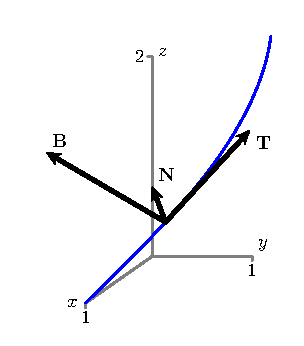
\includegraphics[trim=4.5cm 2.25cm 4.5cm 2.25cm, , clip]{9_8_Ex_4.eps}}
\end{center}
%crop graphics in animate trim=<left> <bottom> <right> <top>,  

	\ea
\end{exerciseSolution}



\item \label{Ez:9.8.5} In this exercise we verify the curvature formula 
\[\kappa = \frac{\lvert \vr'(t) \times \vr''(t) \rvert}{\lvert \vr'(t) \rvert^3}.\]
	\ba
	\item Explain why 
\[\lvert \vr'(t) \rvert = \frac{ds}{dt}.\]

	\item Use the fact that $\vT(t) = \frac{\vr'(t)}{\lvert \vr'(t) \rvert}$ and $\lvert \vr'(t) \rvert = \frac{ds}{dt}$ to explain why 
	\[\vr'(t) = \frac{ds}{dt} \vT(t).\]

	\item The Product Rule shows that 
	\[\vr''(t) = \frac{d^2s}{dt^2} \vT(t) + \frac{ds}{dt} \vT'(t).\]
	Explain why 
	\[\vr'(t) \times \vr''(t) = \left(\frac{ds}{dt}\right)^2 (\vT(t) \times \vT'(t)).\]
	
	\item In Exercise \ref{Ez:9.8.4} we showed that $\lvert \vT(t) \rvert = 1$ implies that $\vT(t)$ is orthogonal to $\vT'(t)$ for every value of $t$. Explain what this tells us about $\lvert \vT(t) \times \vT'(t) \rvert$ and conclude that 
	\[\lvert \vr'(t) \times \vr''(t) \rvert = \left(\frac{ds}{dt}\right)^2 \lvert \vT'(t) \rvert.\]
	
	\item Finally, use the fact that $\kappa = \frac{\lvert \vT'(t) \rvert }{\lvert \vr'(t) \rvert}$ to verify that 
 \[\kappa = \frac{\lvert \vr'(t) \times \vr''(t) \rvert}{\lvert \vr'(t) \rvert^3}.\]
 
	\ea
	
\begin{exerciseSolution}
	\ba
	\item We showed that $\frac{d \vr}{ds} = 1$, so the Chain Rule shows that 
\[\lvert \frac{d \vr}{dt} \rvert = \lvert \frac{d \vr}{ds} \frac{ds}{dt} \rvert = \lvert \frac{d \vr}{ds} \rvert \lvert \frac{ds}{dt} \rvert = \lvert \frac{ds}{dt} \rvert = \frac{ds}{dt},\]
since $s$ is an increasing function. 

	\item Note that 
\[\vr'(t) = \lvert \vr'(t) \rvert \vT(t) = \frac{ds}{dt} \vT(t).\]

	\item Using the previous results we see that 
\begin{align*}
\vr'(t) \times \vr''(t) &= \left( \frac{ds}{dt} \vT(t) \right) \times \left( \frac{d^2s}{dt^2} \vT(t) + \frac{ds}{dt} \vT'(t) \right) \\
	&= \left( \frac{ds}{dt} \vT(t) \times \frac{d^2s}{dt^2} \vT(t) \right) + \left( \frac{ds}{dt} \vT(t) \times \frac{ds}{dt} \vT'(t) \right) \\
	&= \left( \frac{ds}{dt} \right) \left( \frac{d^2s}{dt^2} \right) \left( \vT(t) \times \vT(t) \right) + \left( \frac{ds}{dt} \right) \left( \frac{ds}{dt} \right) \left( \vT(t) \times \vT'(t) \right) \\
	&= \left(\frac{ds}{dt}\right)^2 (\vT(t) \times \vT'(t)).
\end{align*}

	\item We know that 
\[\vT(t) \times \vT'(t) = \lvert \vT(t) \rvert \lvert \vT'(t) \rvert \sin\left(\frac{\pi}{2}\right) \vn\]
for some unit vector $\vn$ orthogonal to both $\vT(t)$ and $\vT'(t)$. So 
\[\lvert \vT(t) \times \vT'(t) \rvert = \lvert \vT(t) \rvert \lvert \vT'(t) \rvert \sin\left(\frac{\pi}{2}\right) \lvert \vn \rvert = \lvert \vT'(t) \rvert.\]
It follows that 
\[\lvert \vr'(t) \times \vr''(t) \rvert = \left(\frac{ds}{dt}\right)^2 \lvert \vT(t) \times \vT'(t) \rvert = \left(\frac{ds}{dt}\right)^2 \lvert \vT'(t) \rvert.\]

	\item We have 
 \[\lvert \vT'(t) \rvert = \frac{\lvert \vr'(t) \times \vr''(t) \rvert}{\left(\frac{ds}{dt}\right)^2}\]
 and so
 \begin{align*}
\kappa &= \frac{\lvert \vT'(t) \rvert }{\lvert \vr'(t) \rvert} \\
	&= \frac{\lvert \vr'(t) \times \vr''(t) \rvert }{\left(\frac{ds}{dt}\right)^2 \lvert \vr'(t) \rvert} \\
	&= \frac{\lvert \vr'(t) \times \vr''(t) \rvert }{\left( \lvert \vr'(t) \rvert \right)^2 \lvert \vr'(t) \rvert} \\
	&= \frac{\lvert \vr'(t) \times \vr''(t) \rvert}{\lvert \vr'(t) \rvert^3}.
\end{align*}

	\ea
\end{exerciseSolution}


\end{exercises}

\afterexercises


\clearpage